\normalsize

\section{Swappable Fields: Proof}
\label{appendix:proof}

\begin{proof}
  Let $F_x$ and $F_y$ be two input fields and their corresponding regular expressions are $RE_x$ and $RE_y$. If $F_x$ and $F_y$ are swappable fields, then $RE_x$ and $RE_y$ have at least two overlapping accepted input.
  \\
  If $F_x$ and $F_y$ are swappable, then 
  $$\exists x_i \in RE_x : x_i \in RE_y\ \text{and}\ \exists y_j \in RE_y : y_j \in RE_x$$ 
  This was the input values $x_i$ and $y_j$ can be swapped.
  Hence, $\{x_i, y_j\} \in RE_x \cap RE_y \Rightarrow |RE_x \cap RE_y| \geq 2$ 
\end{proof}


\section{\tool: Evaluation Details}
\label{appendix:evaluation}

This section provides further details of the \tool evaluation.

\myparagraph{\tool evaluation}
We ran our \tool prototype over several existing configuration web pages from both the PLC server and the home automation system that are listed in Table~\ref{tab:evaluation}. We enumerate the user input fields in each page, their specifications that we manually created (including types and constraints) and the output of the tool that is grouping of swappable fields. We verified each output of the tool manually. We observe that in some cases the tool outputs as ``swappable'' input fields that can, in fact, be easily detected at the server. For example `start date' and `end date' are not swappable as the former has to be less than the later. This is an example of a case, where both fields are specified correctly, but their relationship imposes additional constraints that can be checked by the server. For such type of fields, the developers can exclude them from the input specification.

%% -----------------

%% Tool evaluation table

\begin{table*}[t]
\centering
\caption{\textbf{\tool evaluation.} We tested our implementation of the UI analysis tool on `ControlByWeb x600m' industrial I/O server and `home-assistant' home automation systems. Web pages column shows the configuration pages that we tested. We list types and formats for each user input field in the tested pages, and also list those input fields that are swappable.}
%\footnotesize
\scriptsize
\begin{tabular}{c|lcc|l}
\hline
\textbf{Web pages} & \textbf{Fields} & \textbf{Type} & \textbf{Length/value constraint} &\textbf{Swappable fields} \\
\hline
\multicolumn{5}{c}{\bfseries Web PLC configuration forms} \\
\hline
\multirow{6}{*}{Register configuration} & Name & \String& $[min=1, max=20]$ & Name \\  
 & Description & \String& $[min=0, max=60]$ & Description \\  
 & Type & \integer& $[min=1, max=5]$ & Units \\\cline{5-5}
 & Units & \String& $[min=1, max=5]$ & Decimal place \\  
 & Decimal places & \integer& $[min=0, max=5]$ & Initial  \\  
 & Initial Value & \integer& $[min=0, max=999999]$ & Type\\

\hline
\multirow{7}{*}{Counter configuration} & Device & \radio & \{\texttt{on}, \texttt{off}\} & Name \\ 
 & Device counter number & \integer& $[min=0, max=50]$ & Description\\ \cline{5-5}
 & Name & \String & $[min=1, max=20]$ & Device counter number\\
 & Description & \String & $[min=0, max=60]$ & Decimal places\\
 & Decimal places & \integer & $[min=0, max=5]$ & Debounce \\
 & Debounce & \integer & $[min=0, max=9999]$ & Edge\\ 
 & Edge & \integer & $[min=0, max=6]$ & \\
\hline

\multirow{8}{*}{Event configuration} & Name & \String & $[min=1, max=20]$ & Name\\
 & Description & \String & $[min=0, max=60]$ & Description \\ 
 & Type & \menu & \{\texttt{int}, \texttt{float}, \texttt{boolean}, \texttt{constant}\}& \\ 
 & I/O & \menu & \{available IO\} &\\ 
 & Event group & \menu & \{available Groups\} &\\ 
 & Condition & \menu & \{\texttt{On}, \texttt{Off}, \texttt{Equals}, \texttt{Change state}\}&\\ 
 & Eval on powerup & \radio & \{\texttt{yes}, \texttt{no}\} &\\ 
 & Duration & \integer & $[min=0, max=9999]$ &\\ 
\hline

\multirow{5}{*}{Action configuration} & Name & \String & $[min=1, max=20]$ &Name\\ 
 & Description & \String & $[min=0, max=60]$  &Description \\ 
 & Event source & \menu & \{available events\} &\\ 
 & Type & \menu & \{\texttt{On}, \texttt{Off}, \texttt{Toggle},\ldots\} &\\ 
 & Relay & \menu & \{Available relays\}&\\ 
\hline

\multirow{4}{*}{Supply voltage} & Name & \String & $[min=1, max=20]$ &Name \\ 
 & Description & \String &$[min=0, max=60]$ & Description \\ 
 & Decimal places & \integer & $[min=0, max=5]$ &\\ 
 & Device & \menu & \{Available devices\} &\\
\hline

\multirow{11}{*}{Calendar configuration} & Name & \String & $[min=1, max=20]$ &Name  \\
 & Description & \String & $[min=0, max=60]$ & Description \\ \cline{5-5}
 & Event group & \integer & $[min=0, max=5]$ & Start date  \\ 
 & Start date & \Date & $[min=01/01/2007, max=31/12/2029]$ & Stop date \\ \cline{5-5}
 & Stop date & \Date & $[min=01/01/2007, max=31/12/2029]$ & Start time  \\ 
 & Start time & \Time &  $[min=00:00, max=23:59]$ & Stop time \\ \cline{5-5}
 & Stop time & \Time &   $[min=00:00, max=23:59]$ & Occurrence \\ 
 & All day & \radio & \{\texttt{on}, \texttt{off}\} & Repeat val\\ 
 & Repeat type & \menu & \{None, Secondly, Minutely, \ldots\} & \\ 
 & Repeat val & \integer & $[min=10, max=9999]$ &\\ 
 & Occurrences & \integer & $[min=0, max=999999]$ &\\ 
\hline

\multicolumn{5}{c}{\bfseries Web Home automation configuration forms} \\
\hline

\multirow{6}{*}{Home configuration} & Room door lock & \radio & \rdelim\}{3}{25mm}[{\{\texttt{on}, \texttt{off}\}}] & Room door lock\\
 & Alarm & \radio & &Alarm \\ 
 & Water lawn & \radio && Water lawn\\ 
 & Alarm time & \Time & $[min=00:00, max=23:59]$ &\\ 
 & Nest (thermostat) & \integer & $[min=16, max=25]$&\\ 
 & Sound selection & \menu & \{Available sounds\} &\\  
\hline 

\multirow{5}{*}{Room configuration} & Table lamp & \radio & \rdelim\}{3}{25mm}[{\{\texttt{on}, \texttt{off}\}}] &Table lamp \\
 & TV back light & \radio & &TV back light\\ 
 & Celling lights & \radio & &Celling lights \\ 
 & AC & \integer & $[min=16, max=25]$ &\\ 
 & Window shutter level & \integer & $[min=0, max=10]$ &\\
\hline 
%
\end{tabular}
\vspace{-15pt}
\label{tab:evaluation}
\end{table*}

%%
\myparagraph{Example input fields}
Table~\ref{tab:inputFields} provides provides a listing of additional web UIs that we analyzed using the tool. The list includes web pages for online banking page, medical programmer device, PLC server and home automation system. The main purpose of this table is to provide examples (or templates) for the developer for the fields which they are likely encounter while analyzing with \tool. The table provides the names of the input fields along with their specifications, such as the regular expression and the length/value constraints, and whether some of the fields are mutually swappable or not.

We notice that some user input fields are strictly swappable only with another identical field.  Such as an arbitrary field is not swappable with bank account number such as \emph{IBAN} number due to the specific format (e.g., $[ISO 3166-1\ \text{IBAN code}] [0-9A-Z]^+$ with minimum and maximum length of $20$ and $30$ respectively).



%% -----------------
%% Additional UI specs table

\begin{table*}[t]
\centering
\footnotesize
\caption{\textbf{Input field specifications.} This table lists specifications (type, regular expression, length/value constraints) that we mined by analyzing various web pages (banking, medical, PLC, home automation). The swappable column denotes that the group of input fields with $\checkmark$ mark can be swapped with each other. Such as the current can be swapped with the frequency field.}
\begin{tabular}{lcccl}
\cline{1-5}
\multicolumn{1}{c}{\textbf{Name}} &
\multicolumn{1}{c}{\textbf{Type}} &
\multicolumn{1}{c}{\textbf{Regular expression}} &
\multicolumn{1}{c}{\textbf{Length/value constraints}} & 
\multicolumn{1}{c}{\textbf{Swappable}}
\\
\hline
%\hline\hline
\multicolumn{5}{c}{\bfseries Personal information}\\
\cline{1-5}
Email & \rdelim\}{3}{15mm}[\String] & $(*)^+(@)[a-zA-Z0-9]^+(.)[a-z]^+$ & $[min = 5, max = *]$ & \\
%\cline{1-4}
Name & & $[a-zA-Z.]^+$ & $[min = 1, max = *]$ & \\
%\cline{1-4}
Address & & $[a-zA-Z0-9]^+$ & $[min=5, max=*]$ & \\
%\cline{1-4}
%\cline{1-4}\hline\hline

%\cline{1-4}
%\hline
\cline{1-5}
\multicolumn{5}{c}{\bfseries Medical parameters}\\
\cline{1-5}
Heartbeat & \rdelim\}{3}{15mm}[\integer] & \rdelim\}{3}{3mm}[] \multirow{3}{*}{$[0-9]^+$} & $[min=55,max=210]$ & \rdelim\}{4}{3mm}[$\checkmark$]\\
Blood pressure & & & $[min=80,max=150]$  &\\
Blood sugar (Fasting) & & & $[min=108, max=126]$  &\\
Body temperature & \float & $[0-9]^+((.)[0-9])^*$ & $[min=94,max=108]$ &\\

\cline{1-5}
%\cline{1-4}\hline\hline

\multicolumn{5}{c}{\bfseries Web-based PLC form~\cite{controlbyweb}}\\
\cline{1-5}
Analog Input(voltage) & \rdelim\}{2}{15mm}[\float] & \rdelim\}{2}{3mm}[] \multirow{2}{*}{$[0-9]^+((.)[0-9])^*$} & $[min=0,max=12]$ & \rdelim\}{8}{3mm}[$\checkmark$]\\
Current &  &  & $[min=300 (mA),max=2(A)]$  &\\

Thermocouple & \rdelim\}{6}{15mm}[\integer] & \rdelim\}{6}{3mm}[] \multirow{6}{*}{$[0-9]^+$} & $[min=-15,max=150]$ & \\
Frequency &  &  & $[min=0,max=500(Hz)]$ &\\
Logic repetition &  &  & $[min=0,max=9999]$ &\\
Event duration &  &  & $[min=0, max = 9999999999]$ &\\
Decimal places &  &  & $[min=0, max = 5]$ &\\
Initial value &  &  & $[min=0, max = 999999]$ &\\
%\cline{1-5}
Relay status & \rdelim\}{6}{15mm}[\radio] & \rdelim\}{6}{2mm}[] \multirow{6}{*}{$\{\texttt{On}, \texttt{Off}\}$} & \rdelim\}{6}{3mm}[]\multirow{6}{*}{$[min=0, max=1]$}  & \rdelim\}{6}{3mm}[$\checkmark$]\\
Thermocouple status & &  &   & \\
Thermocouple status &  &   & & \\
Energy slave status &  &  &  & \\
Input module status &  &  &  & \\
Thermostat status &  & & & \\
%\cline{1-5}
Logic start/end date & \Date & $[0-9]^+(/)[0-9]^+(/)[0-9]^+$ & $[min=1/1/2007, max=12/12/2029]$  & \\
%\cline{1-4}
Logic start/end time & \Time & $[0-9]^+(:)[0-9]^+$ & $[min=00:00:00, max=23:59:59]$  & \\
%\cline{1-4}
Logic Script & \rdelim\}{3}{15mm}[\String] & $(*)^+$ & valid controller script & \\
%\cline{1-4}
Module name &  & \rdelim\}{2}{5mm}[]\multirow{2}{*}{$[a-zA-Z0-9]^+$} & $[min=1,max=20]$ & \rdelim\}{2}{3mm}[$\checkmark$]\\
Description &  &  & $[min=0, max = 60]$ &\\

%\cline{1-4}
%\hline
\cline{1-5}
\multicolumn{5}{c}{\bfseries Web-based home automation}\\
\cline{1-5}
Room light toggle & \rdelim\}{4}{15mm}[\radio] & \rdelim\}{4}{2mm}[] \multirow{4}{*}{$$\{\texttt{On}, \texttt{Off}\}$$} & \rdelim\}{4}{3mm}[] \multirow{4}{*}{$[min=0, max=1]$}  & \rdelim\}{4}{3mm}[$\checkmark$]\\
Door lock toggle & & &  &\\
Alarm &  &  &   & \\
A/C &  &  &   & \\
%\cline{1-4}
Room temperature & \rdelim\}{2}{15mm}[\integer] & \rdelim\}{2}{5mm}[]\multirow{2}{*}{$[0-9]^+$} & $[min=6,max=25]$ & \\
%\cline{1-4}
Window shutter level &  &  & $[min=0,max=8]$ & \\
%\cline{1-4}
Alarm time & \Time & $[0-9]^+(:)[0-9]^+$ & $[min=00:00,max=23:59]$ & \\
%\cline{1-4}
\cline{1-5}
\multicolumn{5}{c}{\bfseries Web-based bitcoin wallet~\cite{bitgo,bitcoinwallet,coin,coinbase,blockchain}}\\
\cline{1-5}
\multirow{3}{*}{Address} & \rdelim\}{3}{15mm}[\String] & $[1][P2PKH]^+$ & \rdelim\}{3}{3mm}[]\multirow{3}{*}{$[min=34,max=42]$} & \\
&&$[1][P2SH]^+$&& \\
&&$[bc1][Bech32]^+$&& \\
BTC & \String & $[0-9]^+[.][0.9]^+$ & $[min=0.0,max=9999999999.0]$ & \\
Reference &\String& $[0-9a-zA-Z.-\ ]^*$& $[min=0,max=*]$ & \\

\cline{1-5}
\multicolumn{5}{c}{\bfseries Financial transaction, online banking} \\
\cline{1-5}
IBAN account no. & \String &$(ISO 3166-1\ \text{IBAN code}) [0-9A-Z]^+$ & $[min=20, max=30]$ & \\
%\cline{1-4}
Transaction amount. & \float & $(ISO 4217\ \text{currency code}) [0-9]^+((.)[0-9])^*$ & $[min=0, max=*]$  & \\

\hline
\end{tabular}
\vspace{-20pt}
\label{tab:inputFields}
\end{table*}

%%

\section{User Study: Instructions Sheet}
\label{appendix:userStudy}

%\texttt{\url{https://goo.gl/oMFQBW}} 
Figure~\ref{fig:userStudyInstruction} shows the instruction sheet that we printed and provided to the participants for our user study. The instruction sheet shows a screenshot of the web form, the corresponding instruction, and the actual data that the study participants used in their task. 
%Additionally, we provided a very short introduction to the system and how it can be used in real life. After the participants confirmed that they understand all the written instructions, we started the study. 

%% -----------------
%% User study figure


\begin{figure*}[!h]
 \centering
 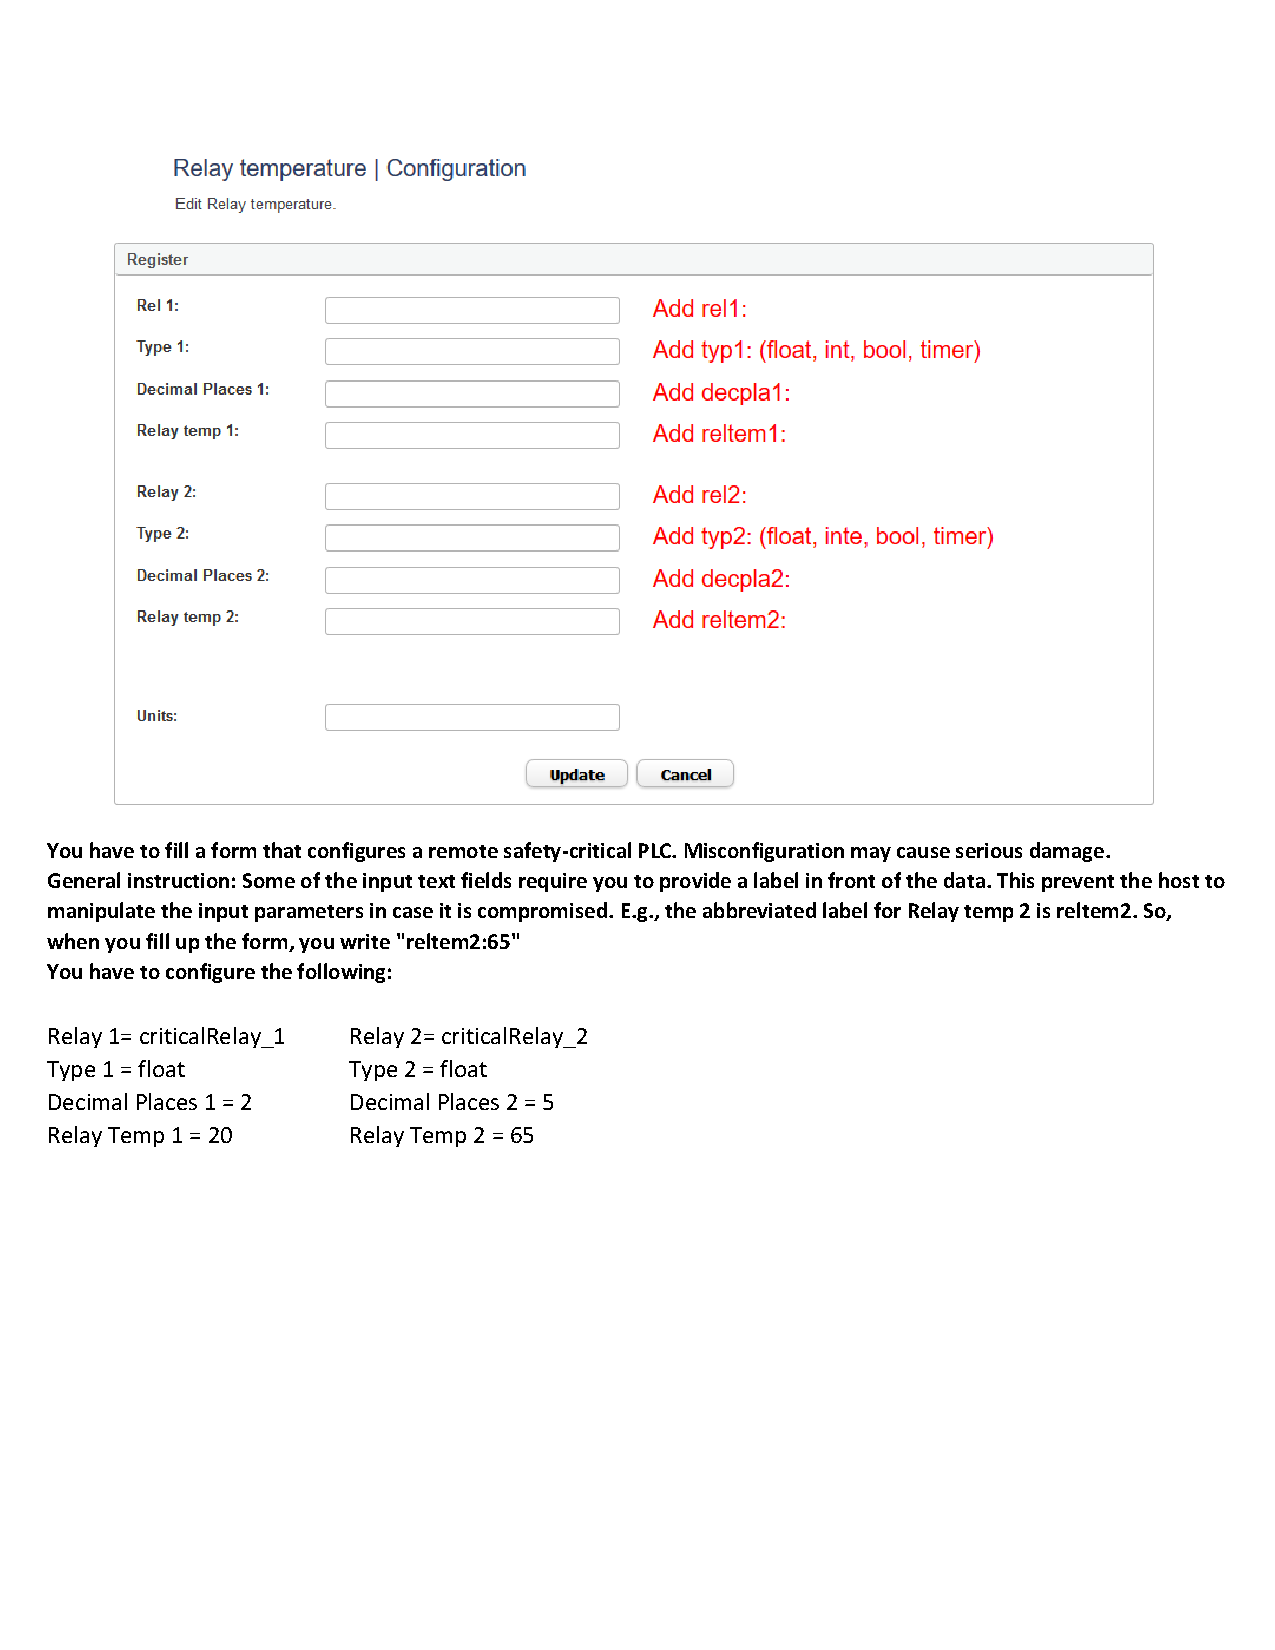
\includegraphics[trim={0 8cm 0 2cm}, clip,width=0.75\linewidth]{userStudy.pdf}
 \caption{\textbf{User study instructions.} This figure shows the instruction sheet that was given to our user study participants.}
 \label{fig:userStudyInstruction}
\end{figure*}

\balance

